\chapter[Introdução]{Introdução}

\section{Problema}

Através da análise das equipes de desenvolvimento, foram identificados aspectos que influenciam no cumprimento de prazos, 
no que diz respeito a entrega de \textit{software}. Esses aspectos foram agrupados e deram origem a causas que ajudaram  a 
identificar o problema de tais equipes.

As seguintes causas foram levantadas:
\begin{itemize}
 \item Baixa produtividade da equipe;
 \item Ineficiência na alocação dos recursos humanos;
 \item Estimativa do tamanho pouco precisa.
\end{itemize}

Portanto, a partir destas causas foi identificado o problema, que são os \textbf{atrasos nas entregas de \textit{software}} 
e para a resolução do mesmo, foi adotada a seguinte questão de pesquisa: \textbf{Quais os aspectos que influenciam a 
entrega no prazo estimado?}.

\vfill
\pagebreak
  
\section{Objetivos}

A partir do diagnóstico realizado nas equipes de desenvolvimento, foi definido como objetivo de negócio \textbf{entregar o 
produto no prazo estimado}.

\subsection{Objetivo Geral}

\begin{itemize}
  \item Conhecer os aspectos que influenciam no cumprimento dos prazos.
\end{itemize}

\subsection{Objetivos Específicos}

\begin{itemize}
  \item Propor um plano de medição.
\end{itemize}

\vfill
\pagebreak

\section{Materiais e métodos}

Para este trabalho primeiramente foi realizada uma revisão de literatura simples
para conhecer mais sobre o assunto tratado, observando pesquisas com problemas semelhantes e
as soluções obtidas.

Como metodologia principal foi utilizada uma pesquisa-ação tendo como objeto de estudo um projeto de uma organização descrita no capítulo \ref{pesquisa_acao}. A pesquisa-ação realizada foi composta das fases representadas na Figura \ref{fig:metodologia}.


\begin{figure}[!htb]
\centering
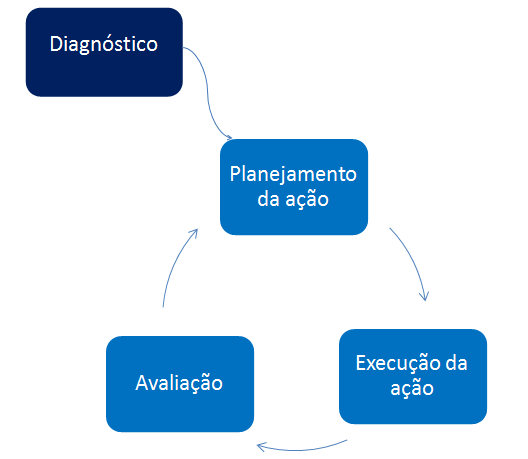
\includegraphics[scale=1]{figuras/pesquisaacao.png}
\caption{Fases da pesquisa-ação. Baseado em \cite{artigo_pesquisa_acao}}
\label{fig:metodologia}
\end{figure}

\pagebreak

De acordo com \citeonline{artigo_pesquisa_acao}, uma pesquisa-ação é composta das seguintes fases:
	\begin{itemize}
		\item \textbf{Diagnóstico:} Essa fase tem como objetivo principal conhecer a situação atual e o problema relacionado ao objeto de estudo. Para realização do diagnóstico foram aplicados questionários.
		\item \textbf{Planejamento da ação:} Essa fase tem como objetivo propor uma ação para resolver o problema diagnosticado, definindo o número de ciclos, as atividades da ação, os envolvidos e como a ação será avaliada.
		\item \textbf{Execução da ação:} Essa fase consiste em executar a ação proposta e acompanhá-la.
		\item \textbf{Avaliação da ação:} Essa fase consiste na avaliação da ação executada a fim de realizar melhorias no próximo ciclo para a ação proposta.
	\end{itemize}

